\documentclass{article}
\usepackage[utf8]{inputenc}
\usepackage{graphicx}
\graphicspath{ {./images/} }

\title{CSE344 HOMEWORK 5 Report}
\author{Can Beyaznar - 161044038}
\date{June 2020}

\begin{document}

\maketitle

\section{Problem Solution}
\paragraph{}
Firstly, while doing the homework, I get the name of the file from the user with
the help of getopt like previous homework. And I do the necessary checks, if
the file cannot be opened, I return an error and end the program. Then, after
making all the checks, I proceed to the file reading process. I have 2 struct
types in the code. One for the client and the other for florists. In the file reading
process, I first find the number of florists and clients in the file, then I define the
florist array and client array that I keep in the global with the help of malloc. Then, by reading the file again, I fill the inside of these arrays with the
information contained in the file. I parse the data in the file line by line. But the
file should definitely come right. After filling these two arrays in the global, I
keep a double-sized array for request queue. The dimensions of this array are
[number of florists] [number of clients]. This array will keep the order of the
orders coming to each florist. And there are the indexes of the clients coming
from the file. While defining this array, I add -1 to each value. Since the number
of florists and clients to be given by the user is uncertain, the locations of all
data are taken with the help of malloc. After doing all these reservation
operations, I define mutex and condition variables that I will use in my threads.
I have defined an array for my mutex. In total, there will be as many mutex as
the number of florists. And each one will be processed only among themselves
in the thread. Because two different florists should not prevent each other from
working. Only main can control mutex as a different location. The same
conditions are valid for condition variables. I allocate as many flower shops as
there are. And each one will wait for the orders coming to it. When these
orders arrive, Main will wake up the condition variable that depends on it with
cwait.
\mbox{}\\

\paragraph{}
After these processes, I move on to create threads. In total, I produce threads
as many as the number of florists, and I send that florist's index to the thread
function to understand which florist is working. After creating these threads, I
go to the main thread section. The loop here continues as many as the number
of clients and I send each client to the request queue. First of all, I get the
information of the client in my current location from my client array. And I
compare the flower name requested by the client with the names of the flowers
in my florists. And I count how many florists have the flower he wants. Then I
reserve a space in an array (index\verb!_!arr) to store the indexes of these florists. And I repeat the same process to keep the florists' indexes. Now that I know
which florists are present, I can find the nearest florist to the client. Here I
calculate Chebyshev distance between each florist and client. And I return the
index of the florist with the minimum distance between them. After I get this
index, I lock the florist of the florist attached to that index. Then I update the
request queue. I go to this index in request queue and assign the client's index
to the last element. Thus, I learn which client to send flowers to the florist. After
updating this array that thread will use, I unlock mutex which is connected to
the florist. Thus, the threads continue to work without any data loss. Also, before I unlock it, I am sending a signal to the condition variable that the florist
is connected (pthread\verb!_!cond\verb!_!signal) because a new order has arrived. Thus,
the florist can continue working as a new order has arrived. This process
continues for the number of clients and all orders are sent to request queue. And the main thread continues to work without interruption. After these
processes are finished, I assign the exitThread parameter to 1. I use this
parameter for my florist threads. Thus, the florists learn that the orders are over, and they place all the orders they have and terminate themselves. When
changing the value of the exitThread parameter, I lock all the mutex that the
florists are connected to, so that there is no deadlock. And after changing the
value of the parameter, I unlock all mutex. After these processes, I am sending
a signal to each condition variable, since there may still be a thread waiting for
the signal. Thus, the florist threads will check the exitThread parameter, see
that the orders are over and write all their orders and exit the function. I am
also waiting for my threads with pthread\verb!_!join to avoid zombie process. And
after each thread is finished, I destroy the mutex and condition variable that
are connected to it. Then, I am free all the parameters I have reserved with
malloc and end the program. If it fails to use thread functions, I warn and end
the program.
\mbox{}\\

\paragraph{}

After explaining the main thread, we can come to the thread where the florists
are. In this thread, I first convert the parameter from main to integer. Thanks to
this parameter, I can find out which florist works. Then I create a loop that
continues as long as the exitThread parameter is 0 (ie, unless the orders are
finished). At the beginning of this cycle I always check to see if orders are
finished. If it is finished, the florist takes all his orders and leaves the program. After providing this control, I check whether the order is available. If there is no
order, this florist should wait for the order to arrive. I do this with the
pthread\verb!_!cond\verb!_!wait function. I am holding this thread using the condition
variable to which the florist is connected. So the main thread can send a signal
to this florist when the order arrives. This loop continues as long as no current
order is received and orders are not finished. After leaving this cycle, we face
two possibilities. If the main thread has read all the orders, the florist will
deliver all the orders attached to it and terminate the program. If the orders are
not finished, the florist takes the order and delivers it. I lock the mutex to which
the florist is connected to avoid any problems when changing the value of the
parameters used by the main thread. And at the end of the process, I remove
the lock. And if the florist thread ends, I print a message saying that it closed
the shop. When delivering, I first generate a random number between 1-250
(for sleep). Then I determine the distance between the florist and the client with
Chebyshev Distance. Then I divide this distance to the florist's ms to calculate
the order time. And I add this result by the random number I produced for sleep. So I calculate the elapsed time for an order. Before I write the required
information on the screen, I sleep in milliseconds with the usleep function. These procedures are the same for all florists. Main thread waits for the
delivery of all florists. And after it is done, it destroys the thread related data. And it frees all the data separated by malloc. After delivery, general
information of florists is printed.
\mbox{}\\
\paragraph{About Ctrl C (SIGINT) signal}

If we come to the handle of SIGINT signal, I would handle this with the help of sigaction in main. If SIGINT signal comes, I go to my signalhandler function and set the exitThread parameter to -1. And I check the exitThread parameter inside my florist threads. If this parameter is equal to -1, I get out of that thread. And I also check the exitThread parameter first, when the threads are writing messages on the screen. If it is equal to -1, I prevent him from writing the message. In the Main part, I just prevent it from writing the information it will write on the screen. Thus, threads can exit the program when appropriate. If I wait for threads in the signalhandler function, errors can occur and memory leaks can occur. That is why I am changing only one parameter, so that it works without breaking the structure of the program. And so when the SIGINT signal comes from the user, it continues to do some things that the main thread and florist threads need to do, and terminates the program at the appropriate time.
\mbox{}\\

\newpage
\paragraph{}
The structures that I keep the information of the client and florist are as follows.

\mbox{}\\
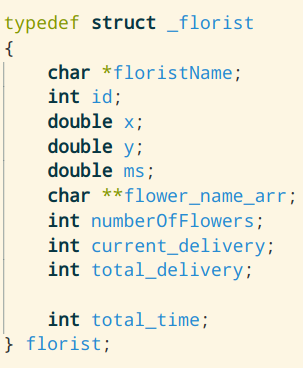
\includegraphics[width=6cm, height=6cm]{v1.png}
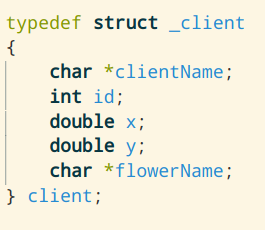
\includegraphics[width=6cm, height=6cm]{v2.png}
\mbox{}\\

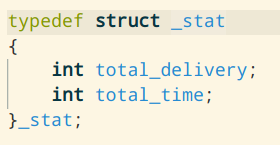
\includegraphics[width=6cm, height=4cm]{v3.png}
\paragraph{Note}
stat structure is used to print the information returned by the thread

\section{Output Example}
    \subsection{Data.dat}
    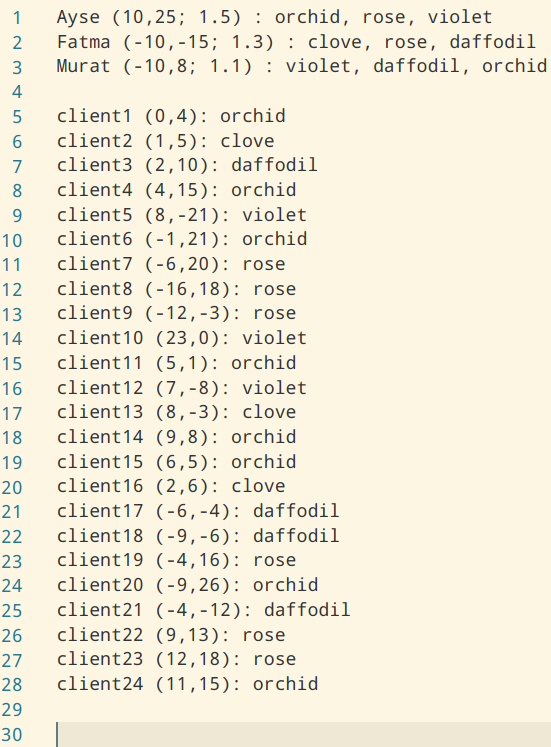
\includegraphics{datadat.png}
    
    \subsection{makefile}
    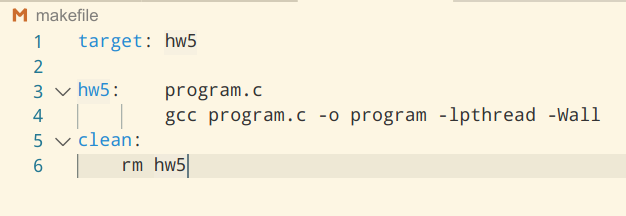
\includegraphics{makefile.png}
    
    \subsection{output}
    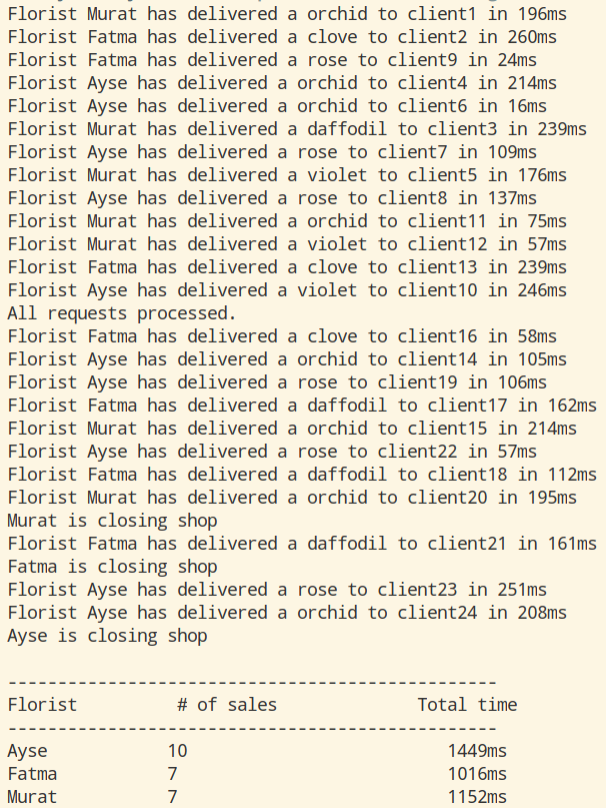
\includegraphics{output.png}

\end{document}
